\documentclass[floatfix]{article}
\usepackage[utf8x]{inputenc}
\usepackage[pdftex]{graphicx}
\usepackage{mathpazo} 
\usepackage{amsmath}
\usepackage{amsfonts}
\usepackage{amssymb}
\usepackage{braket}
\usepackage{dsfont}
\usepackage[pdftex]{hyperref}   
\usepackage{siunitx}
\usepackage{bbm, dsfont}
\usepackage[font=small]{caption}
\usepackage[margin=1in]{geometry}
\usepackage{float}
\usepackage{tikz}
\usetikzlibrary{arrows,shapes,trees}
\usepackage{media9}

\newcommand*{\gd}{
\textcolor{green}{\ast}}

\newcommand*{\md}{
\textcolor{magenta}{\ast}}

\newcommand*{\ud}{
\underline{\space\space}}

\graphicspath{{images/},{figures/}}

\title{Systems with a strong interaction to an enviroment}
\author{Eduardo Villase\~nor \\ Carlos Gonzales}
\date{\today}

\begin{document}
\maketitle



\section{Transitions in the P(s)}

We are interested in finding the transitions of from a GOE to Poisson statistics on the
nearest neighbour distribtion ($P(s)$) when the parameters change from the ergodic regime to the non-ergodic 
one.

Spectra was obtained with two diferent methods, in the first one we break the symetrie by varying the Ising interaction between the
spins on the closed chain. For the second one we decomposed the open chain into reflection symmetrie sectors.

Animations of the $P(s)$ for a chain in the two cases varying different componentes of the magnetic kick. As
the color lines in the Fig. \ref{anim_gui} shows.

\begin{figure}[H]
\begin{center}
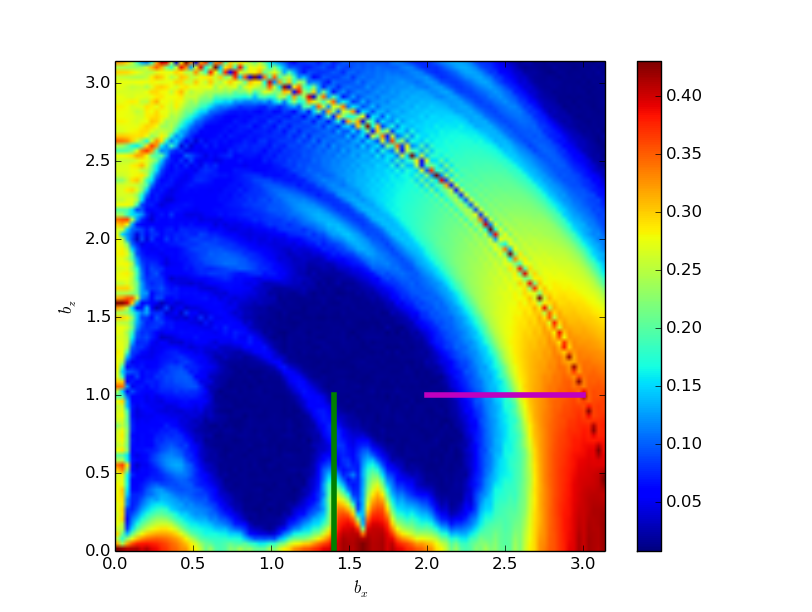
\includegraphics[width=.5\columnwidth]{anim_guide}  
\end{center}
\caption{}
\label{anim_gui}
\end{figure}

The animations are ass follows 
\begin{itemize}
\item ``Ps\ud transition1" - Closed chain $J=1$ $b_x=[2,3]$ $b_z=1.$ $\Delta J = 0.1$ $\md$
\item ``Ps\ud transition1\underline{\space\space}sym" - Open chain $J=1$ $b_x=[2,3]$ $b_z=1.$ reflection symetries used $\md$
\item ``Ps\ud transition2" - Closed chain $J=1$ $b_x=1.4$ $b_z=[0,1]$ $\Delta J = 0.1$ $\gd$
\item ``Ps\ud transition2\underline{\space\space}sym" - Closed chain $J=1$ $b_x=1.4$ $b_z=[0,1]$ reflection symetries used $\gd$
\end{itemize}


\section{Purity decay}

\end{document}